\chapter{Ottica geometrica}%Ottica geometrica
\section{Leggi della riflessione e della trasmissione}%Leggi della riflessione e della trasmissione
Si ricordano le leggi della \b{riflessione}:
\begin{equation}\begin{split}
\theta_i=\theta_r
\end{split}\end{equation}
e della \b{rifrazione}
\begin{equation}\begin{split}
\frac{\sin{\theta_t}}{\sin{\theta_i}}=\frac{\n1}{\n2}.
\end{split}\end{equation}

La definizione di \b{indice di rifrazione} è:
\begin{equation}\begin{split}
n=\frac{c}{v}
\end{split}\end{equation}
e di \b{angolo limite}:
\begin{equation}\begin{split}
\theta_L=\arcsin{\frac{\n2}{\n1}}
\end{split}\end{equation}
che descrive il fenomeno della \b{riflessione totale}:
\begin{equation}\begin{split}
\sin{\theta_L}=\frac{\n2}{\n1}.
\end{split}\end{equation}

\section{Definizioni e convenzioni}%Definizioni e convenzioni
Fissata una superficie di discontinuità e detto $V$ il suo vertice, cioè l'intersezione con l'asse ottico che coincide con l'asse di simmetria ci si attiene alle seguenti regole:
\begin{center}
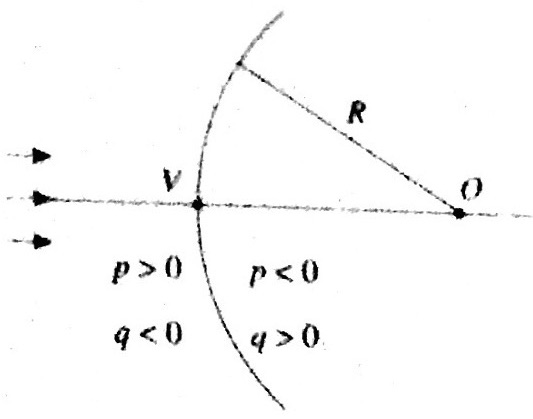
\includegraphics[width=2in]{immagini/otticgeom1.jpg}
\end{center}
\begin{center}
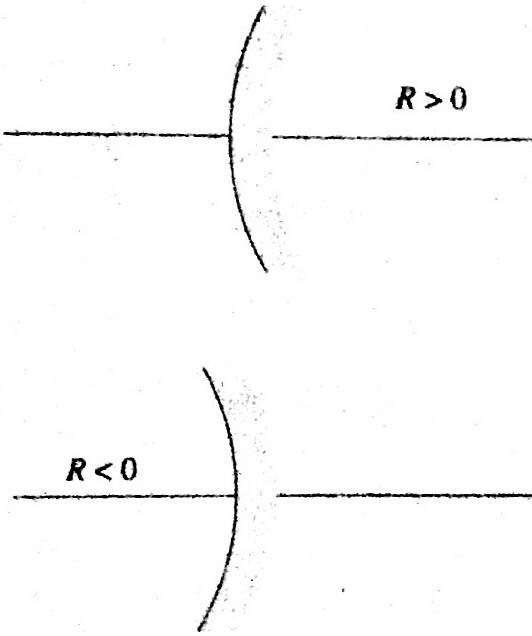
\includegraphics[width=2in]{immagini/otticgeom2.jpg}
\end{center}
\begin{itemize}
\item la luce incidente proviene da sinistra;
\item la distanza $p$ di un oggetto $P$ dal vertice $V$ è positiva se l'oggetto si trova a sinistra del vertice, negativa se l'oggetto è a destra;
\item la distanza $q$ dell'immagine $Q$ dal vertice $V$ è positiva se l'oggetto si trova a destra del vertice, negativa se l'oggetto è a sinistra;
\item il raggio di curvatura $R$ della superficie sferica è positivo se il centro di curvatura si trova a destra di $V$ (convesso), negativo se il centro di curvatura è a sinistra di $V$ (concavo);
\item a sinistra di $V$ gli angoli che i raggi formano con l'asse sono positivi se considerati nel verso antiorario a partire dall'asse, a destra di $V$ il verso positivo è quello orario;
\item le distanze dall'asse sono positive per punti al di sopra dell'asse, negative per punti al di sotto, se si tratta di oggetti; per le immagini vale il contrario.
\end{itemize}
\begin{center}
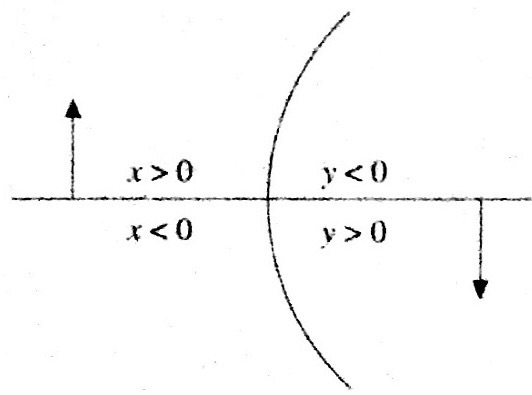
\includegraphics[width=2in]{immagini/otticgeom3.jpg}
\end{center}

\subsubsection{Specchi}
Le superfici che la luce incontra sono dette catottriche o specchi quando su di esse avviene solo la riflessione. I raggi di qualsiasi lunghezza d'onda propagantesi nella stessa direzione subiscono tutti la stessa deviazione.

\subsubsection{Diottri}
Le superfici su cui avviene la rifrazione della luce da un mezzo all'altro sono dette superfici diottriche o diottri. I raggi propagantisi nella stessa direzione con diversa lunghezza d'onda subiscono deviazioni diverse. Di un unico oggetto si possono avere più immagini distinte e colorate e il sistema non è quindi stigmatico. Questo difetto intrinseco si chiama \b{cromatismo}.

\section{Specchi}%Specchi
Lo \b{specchio piano} è \b{stigmatico e aplanatico} senza alcuna limitazione ed è l'unico strumento ad avere queste proprietà unite all'\b{acromaticità}.

Gli \b{specchi sferici}, anch'essi \b{acromatici}, sono \b{stigmatici e aplanatici} solo \b{in approssimazione}.
\subsection{Specchio sferico concavo}
\begin{center}
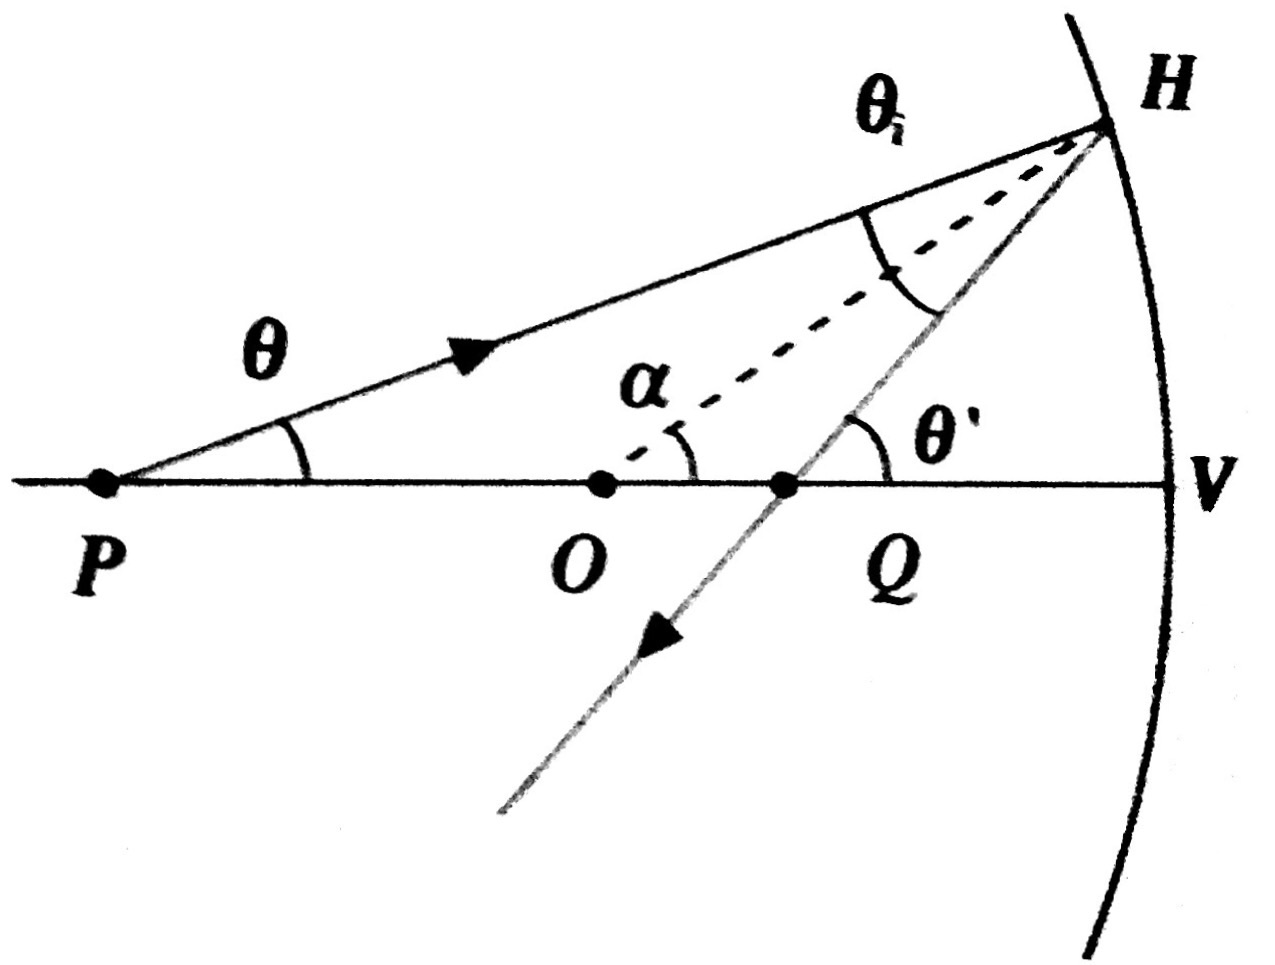
\includegraphics[width=2in]{immagini/specchi1.jpg}
\end{center}

Si pone un oggetto $P$ puntiforme sull'asse dello specchio a sinistra del centro di curvatura $O$ e si traccia un raggio emesso da $P$ ad un angolo $\theta$ con l'asse. Il raggio incide sullo specchio nel punto $H$ e il raggio riflesso incontra l'asse nel punto $Q$, immagine di $P$. Si ha quindi una \b{relazione sempre valida}:
\begin{equation}\begin{split}
\theta+\theta'=2\alpha
\end{split}\end{equation}
considerando $\theta$ l'angolo in $P$, $\theta'$ l'angolo in $Q$ e $\alpha$ l'angolo in $O$.

Supponendo che gli angoli siano piccoli, si ottiene che l'arco $HV$ può essere confuso con il segmento perpendicolare da $H$ all'asse, e quindi:
\begin{equation}\begin{split}
h=PV\tan{\theta}=PV\theta, \qquad h=HV\theta', \qquad h=OV\alpha
\end{split}\end{equation}
che portano a:
\begin{equation}\begin{split}
PV=p, \qquad QV=-q, \qquad OV=-R\\
\theta=\frac{h}{p}, \qquad \theta'=-\frac{h}{q}, \qquad \alpha=-\frac{h}{R}
\end{split}\end{equation}
Si ottiene quindi l'\b{equazione dello specchio sferico concavo nell'approssimazione parassiale}:
\begin{equation}\begin{split}
\frac{1}{p}-\frac{1}{q}=-\frac{2}{R}=-\frac{1}{f}
\end{split}\end{equation}
che mostra come \b{nell'approssimazione parassiale lo specchio concavo è stigmatico}.

\subsubsection{Formazione dell'immagine}
\begin{center}
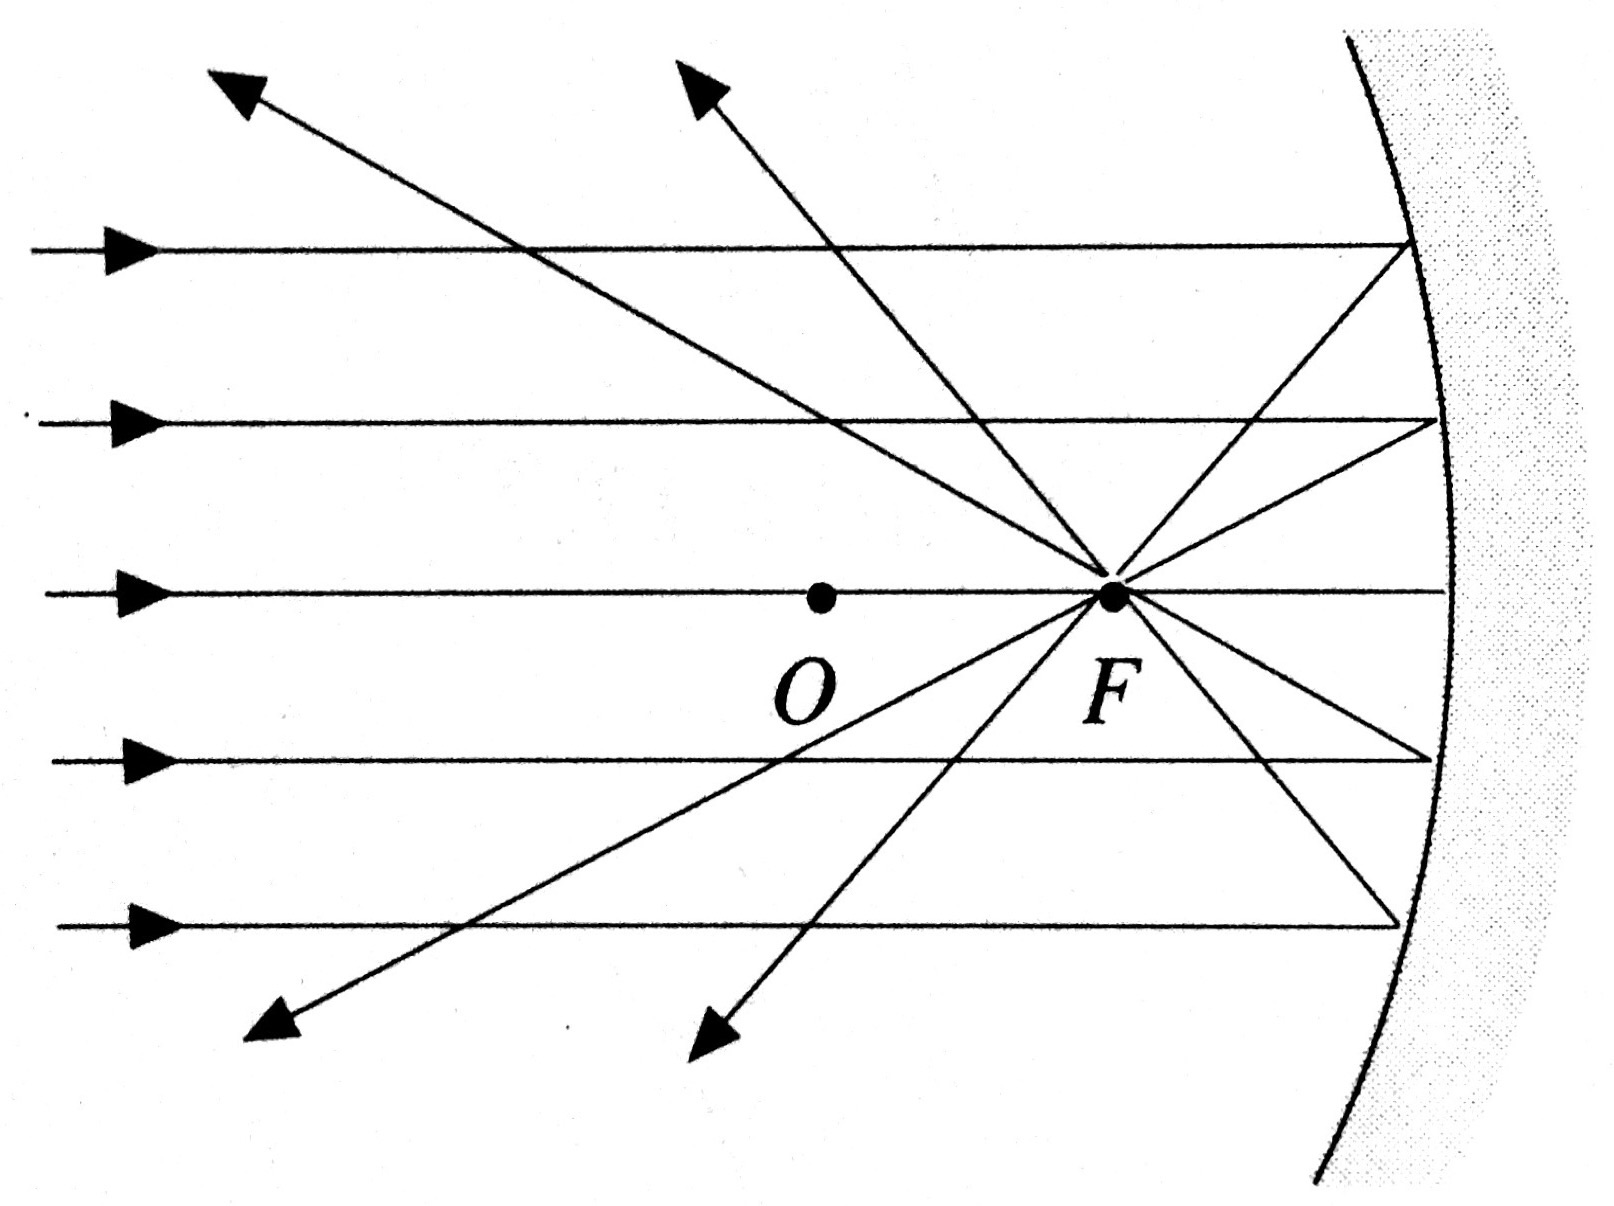
\includegraphics[width=2in]{immagini/specchi2.jpg}
\end{center}

Considerando $p=+\infty$ si ottiene:
\begin{equation}\begin{split}
q=\frac{R}{2}=f
\end{split}\end{equation}
denominando $f=-FV$ la \b{distanza focale} e il \b{fuoco} $F$ il punto d'incontro dei raggi.

Quando $P$ si avvicina al centro di curvatura $O$, $Q$ si sposta da $F$ verso $O$. Se $P$ è posto in $O$, anche $Q$ cade in $O$. Quando $P$ si sposta da $O$ a $F$, $Q$ si sposta da $O$ verso $-\infty$. Quando l'oggetto è nel fuoco ($p=-f$) l'immagine si forma all'infinito e i raggi riflessi sono paralleli all'asse. Questi sono esempi di \b{immagine reale}.

Quando $P$ si trova tra il fuoco $F$ e il vertice $V$, l'immagine $Q$ si forma oltre lo specchio: i raggi riflessi sembrano provenire da $Q$ e ciò vuol dire che per $P$ compreso tra fuoco e vertice l'\b{immagine è virtuale}.

Se l'oggetto è \b{reale}, cioè se la luce che colpisce lo specchio diverge da un punto posto sull'asse, l'immagine può essere reale, situata tra $-\infty$ e $F$, oppure virtuale, situata tra $V$ e $+\infty$. Se l'oggetto è \b{virtuale}, cioè se la luce che colpisce lo specchio converge da un punto posto sull'asse, l'immagine è reale e si forma tra il fuoco $F$ e il vertice $V$.

\begin{center}
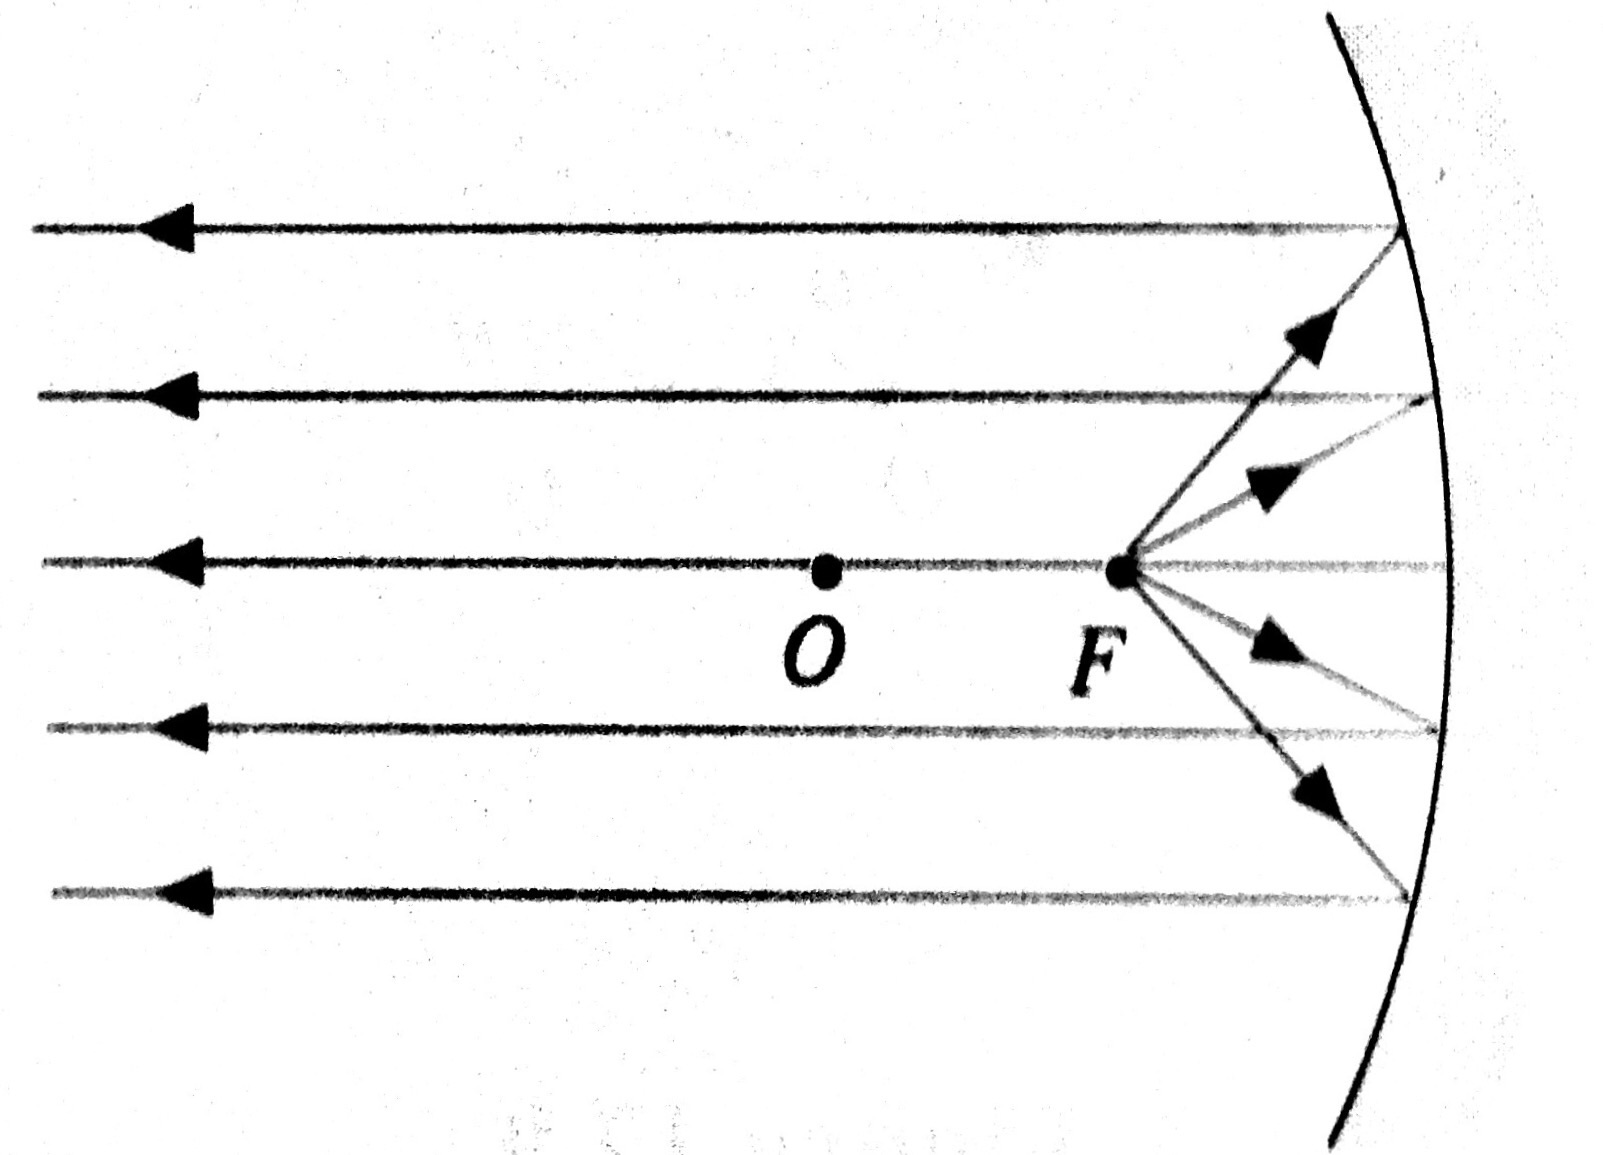
\includegraphics[width=2in]{immagini/specchi3.jpg}
\end{center}
\begin{center}
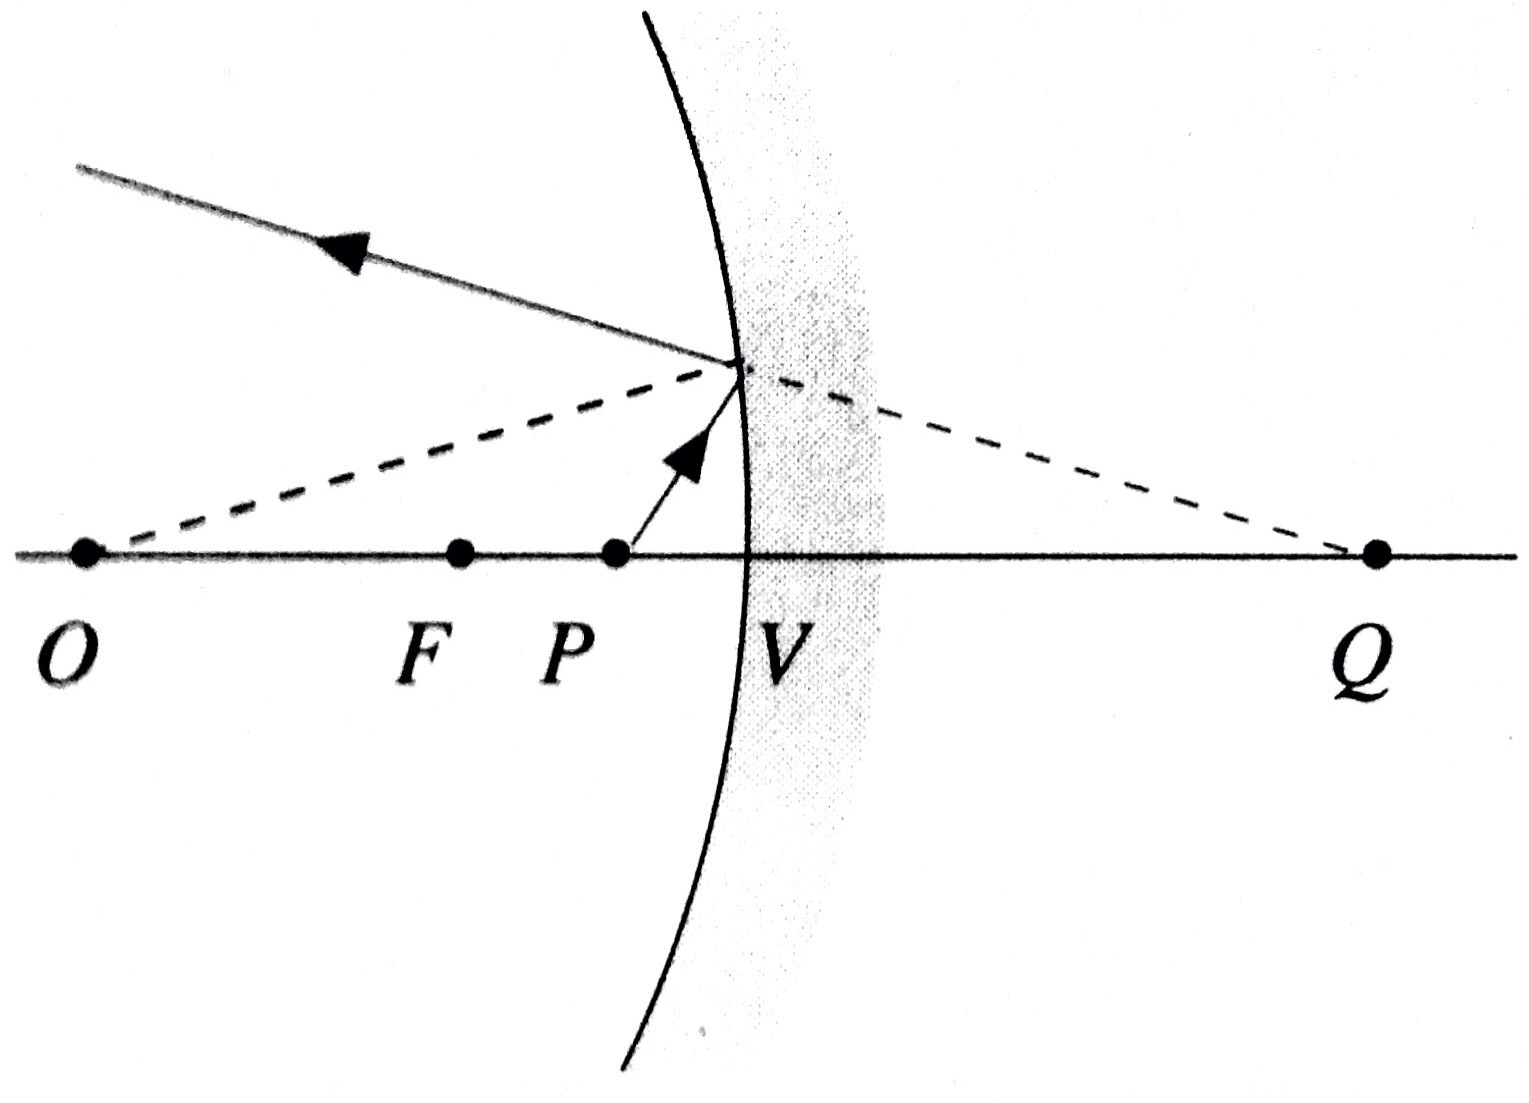
\includegraphics[width=2in]{immagini/specchi4.jpg}
\end{center}

\subsubsection{Relazioni tra oggetto e immagine}
\begin{center}
\begin{tabularx}{\textwidth}{Xc| Xc}
\toprule
\multicolumn{2}{c}{Oggetto} 			& \multicolumn{2}{c}{Immagine} 	\\
\midrule
$+\infty\ge p\ge-R$ 		& reale 		& $\frac{R}{2}\ge q\ge R$ 		& reale\\[2ex]
$-R\ge p\ge -\frac{R}{2}$ 	& reale 		& $R\ge q\ge -\infty$ 			& reale\\[2ex]
$-\frac{R}{2}\ge p\ge 0$ 	& reale 		& $+\infty\ge q \ge 0$ 			& virtuale\\[2ex]
$0> p\ge -\infty$ 		& virtuale 		& $0\ge q\ge \frac{R}{2}$ 		& reale\\[2ex]
\bottomrule
\end{tabularx}
\end{center}

\b{Quando l'immagine è reale, essa è capovolta rispetto all'oggetto, mentre l'immagine virtuale risulta diritta}.

La luce emessa da un punto $F'$ che sta nel piano ortogonale all'asse passante per il fuoco $F$ dopo la riflessione forma un fascio di raggi paralleli tra loro; se la distanza tra $F$ e $F'$ è $d$, si ha $d=|f|\theta$. Un fascio di raggi paralleli provenienti da infinito, invece, si incontra dopo la riflessione nel punto $F'$. Il luogo dei punti $F'$ così individuati si chiama \b{piano focale}.

\begin{center}
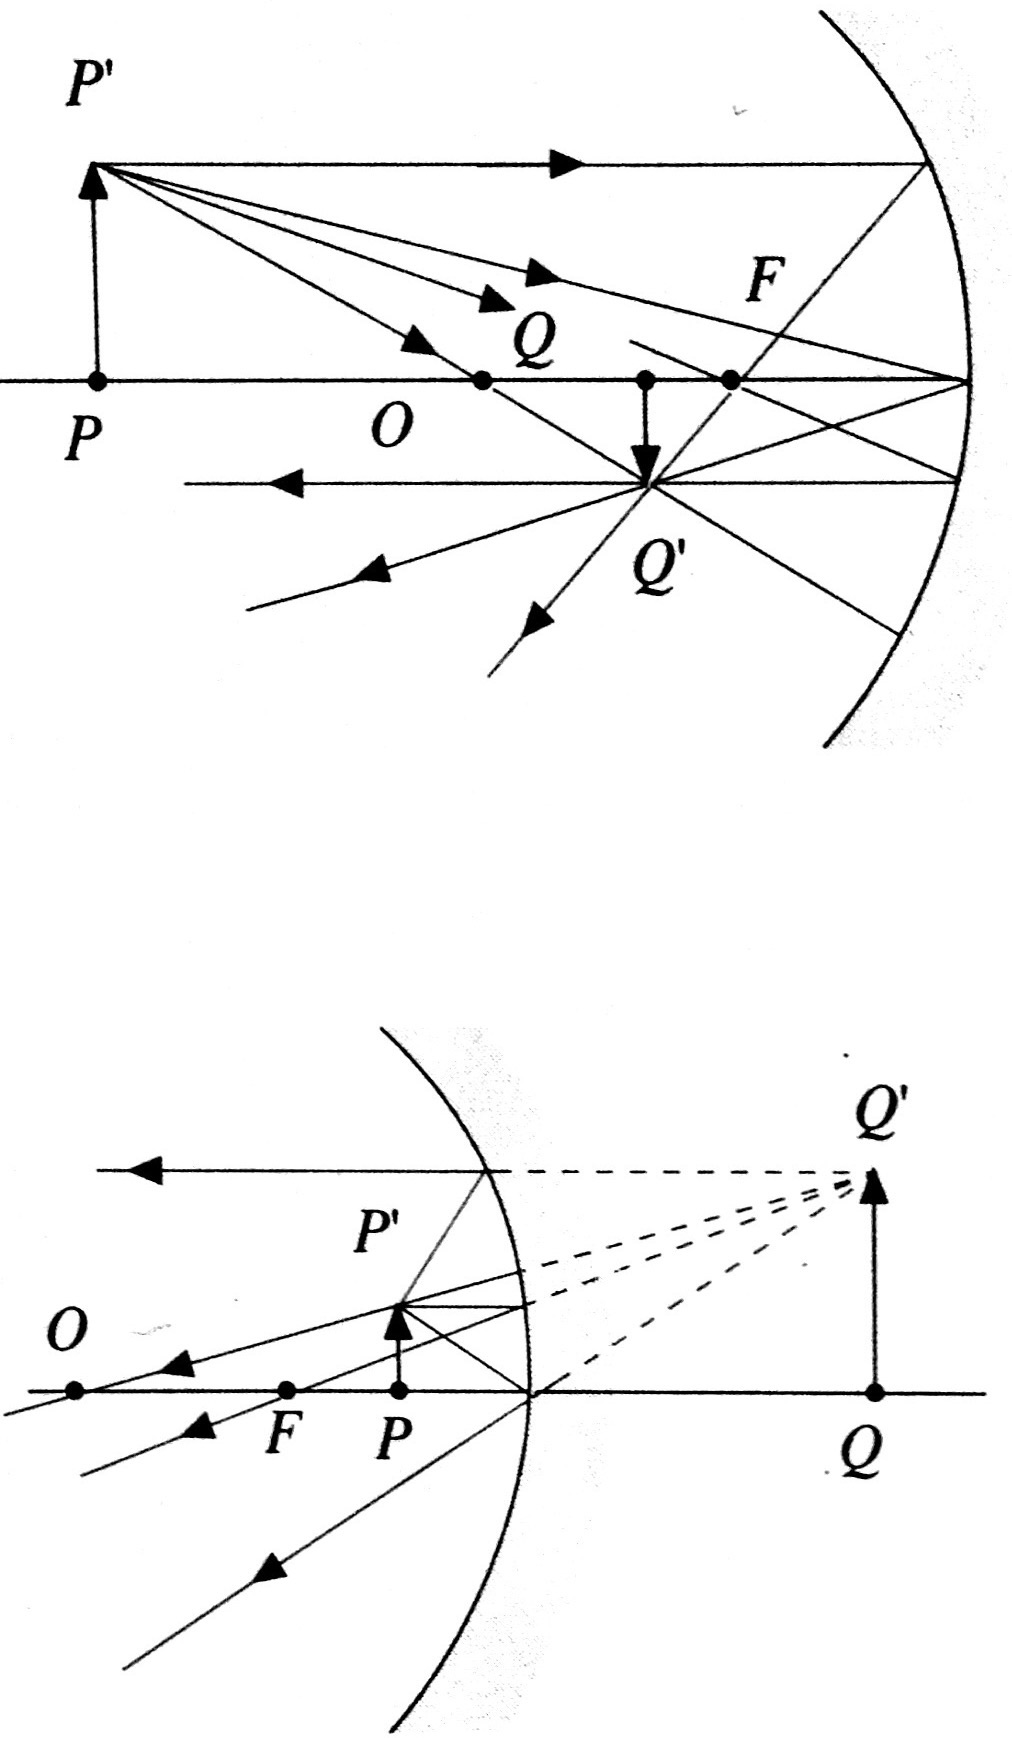
\includegraphics[width=2in]{immagini/specchi5.jpg}
\end{center}

L'\b{ingrandimento trasversale} dello specchio sferico viene definito come:
\begin{equation}\begin{split}
\In=\frac{y}{x}
\end{split}\end{equation}
che può essere vista anche come:
\begin{equation}\begin{split}
\In=\frac{q-R}{p+R}=-\frac{R}{2p+R}=-\frac{f}{p+f}=\frac{2q-R}{R}=\frac{q-f}{f}=-\frac{q}{p}
\end{split}\end{equation}
la quale porta a diversi casi:
\begin{equation}\begin{split}
\begin{cases}
\textrm{immagine capovolta e rimpicciolita}, & 1\ge\In\ge0\\
\textrm{immagine capovolta e ingrandita}, & \In\ge1\\
\textrm{immagine diritta e ingrandita}, & \In<-1\\
\textrm{immagine diritta e rimpicciolita}, & -1<\In\le0
\end{cases}
\end{split}\end{equation}

\subsection{Specchio sferico convesso}
Per questo tipo di specchi basta ruotare di \ang{180;;} lo specchio concavo e i relativi risultati e si rende speculare la faccia convessa della superficie che guarda verso sinistra e si scambia l'oggetto con l'immagine.

Si ottiene quindi l'\b{equazione dello specchio sferico convesso nell'approssimazione parassiale}:
\begin{equation}\begin{split}
\frac{1}{p}-\frac{1}{q}=\frac{2}{R}=\frac{1}{f}.
\end{split}\end{equation}

\subsubsection{Relazioni tra oggetto e immagine}
\begin{center}
\begin{tabularx}{\textwidth}{Xc| Xc}
\toprule
\multicolumn{2}{c}{Oggetto} 			& \multicolumn{2}{c}{Immagine} 	\\
\midrule
$+\infty\ge p> 0$ 		& reale 		& $\frac{R}{2}\ge q\ge 0$ 		& virtuale\\[2ex]
$0\ge p\ge -\frac{R}{2}$ 	& virtuale 		& $0\ge q\ge -\infty$ 			& reale\\[2ex]
$-\frac{R}{2}\ge p\ge -R$ 	& virtuale 		& $+\infty\ge q \ge R$ 			& virtuale\\[2ex]
$-R \ge p\ge -\infty$ 		& virtuale 		& $R\ge q\ge \frac{R}{2}$ 		& virtuale\\[2ex]
\bottomrule
\end{tabularx}
\end{center}

\subsection{Specchio piano}
\'E il caso limite dello specchio concavo per $R\to-\infty$: il fuoco va all'infinito, l'oggetto è sempre tra fuoco e vertice e l'immagine è sempre virtuale. Si ha l'\b{equazione dello specchio piano}:
\begin{equation}\begin{split}
p=q.
\end{split}\end{equation}

\section{Diottri}%Diottri
\subsection{Diottro sferico convesso}
Si suppone $\n1<\n2$. Le relazioni tra gli angoli sono:
\begin{equation}\begin{split}
\theta+\alpha=\theta_i, \qquad \theta_t+\theta'=\alpha\\
\Longrightarrow \n1\theta+\n2\theta'=\(\n2-\n1\)\alpha.
\end{split}\end{equation}
Si ha che tutti gli angoli $R$, $p$ e $q$ sono positivi e pertanto essendo $h=HV=HK$ si ha:
\begin{equation}\begin{split}
\theta=\frac{h}{p}, \qquad \theta'=\frac{h}{q}, \qquad \alpha=\frac{h}{R}
\end{split}\end{equation}
essendo $\theta$ l'angolo in $P$, $\theta$ l'angolo in $Q$ e $\alpha$ l'angolo in $O$.

Si ha l'\b{equazione del diottro sferico convesso nell'approssimazione parassiale}:
\begin{equation}\begin{split}
\frac{\n1}{p}+\frac{\n2}{q}=\frac{\n2-\n1}{R}\\
\frac{f_1}{p}+\frac{f_2}{q}=1
\end{split}\end{equation}
chiamando \b{potere convergente} il valore $\frac{\n2-\n1}{R}$.

Quando l'\b{oggetto è posto a distanza infinita} ($p=+\infty$) si ha che l'immagine si forma oltre il vertice a distanza:
\begin{equation}\begin{split}
f_2=\frac{\n2R}{\n2-\n1}
\end{split}\end{equation}
nel \b{fuoco posteriore} del diottro $F_2$.

Quando l'\b{immagine si forma all'infinito} ($q=+\infty$) si ha che l'immagine si forma oltre il vertice a distanza:
\begin{equation}\begin{split}
f_1=\frac{\n1R}{\n2-\n1}
\end{split}\end{equation}
nel \b{fuoco anteriore} del diottro $F_1$.

\subsubsection{Relazioni tra oggetto e immagine}
\begin{center}
\begin{tabularx}{\textwidth}{Xc| Xc}
\toprule
\multicolumn{2}{c}{Oggetto} 			& \multicolumn{2}{c}{Immagine} 	\\
\midrule
$+\infty\ge p\ge f_1$ 		& reale 		& $f_2\le q\le +\infty$ 			& reale\\[2ex]
$f_1\ge p\ge 0$ 			& reale 		& $-\infty\le q\le 0$ 			& virtuale\\[2ex]
$0\ge p\ge -\infty$ 		& virtuale 		& $0\le q \le f_2$ 			& reale\\[2ex]
\bottomrule
\end{tabularx}
\end{center}

\b{Nei diottri convergenti i fuochi sono reali mentre in quelli divergenti i fuochi sono virtuali e le loro posizioni sono scambiate}: $F_1$ è a destra del vertice, $F_2$ è a sinistra. I piani ortogonali all'asse nei punti $F_1$ e $F_2$ si chiamano \b{piani focali}: i loro punti sono le immagini di punti all'infinito che inviano un fascio di raggi paralleli tra loro e ad un certo angolo con l'asse.

Vengono definiti infine l'\b{ingrandimento trasversale}:
\begin{equation}\begin{split}
\In=\frac{y}{x}=\frac{q-R}{p+R}=\frac{f_1}{p-f_1}=\frac{q-f_2}{f_2}=\frac{\n1q}{\n2p}
\end{split}\end{equation}
e l'\b{ingrandimento longitudinale}:
\begin{equation}\begin{split}
\frac{\Delta q}{\Delta p}=\frac{q_2-q_1}{p_2-p_1}=-\frac{\n2}{\n1}I_1I_2\\
\Longrightarrow \frac{dq}{dp}=-\frac{\n2}{\n2}I^2.
\end{split}\end{equation}

\subsection{Diottro piano}
Se il raggio della superficie diottrica tende all'infinito il diottro diventa piano e si ha l'\b{equazione del diottro piano}:
\begin{equation}\begin{split}
q=\frac{\n2}{\n1}p.
\end{split}\end{equation}

Un oggetto reale dà sempre un'immagine virtuale mentre un oggetto virtuale dà sempre un'immagine reale; il potere diottrico è nullo, l'ingrandimento trasversale è $-1$ e quello longitudinale è $-\frac{\n2}{\n1}$.

\section{Lenti sottili}%Lenti sottili
\begin{center}
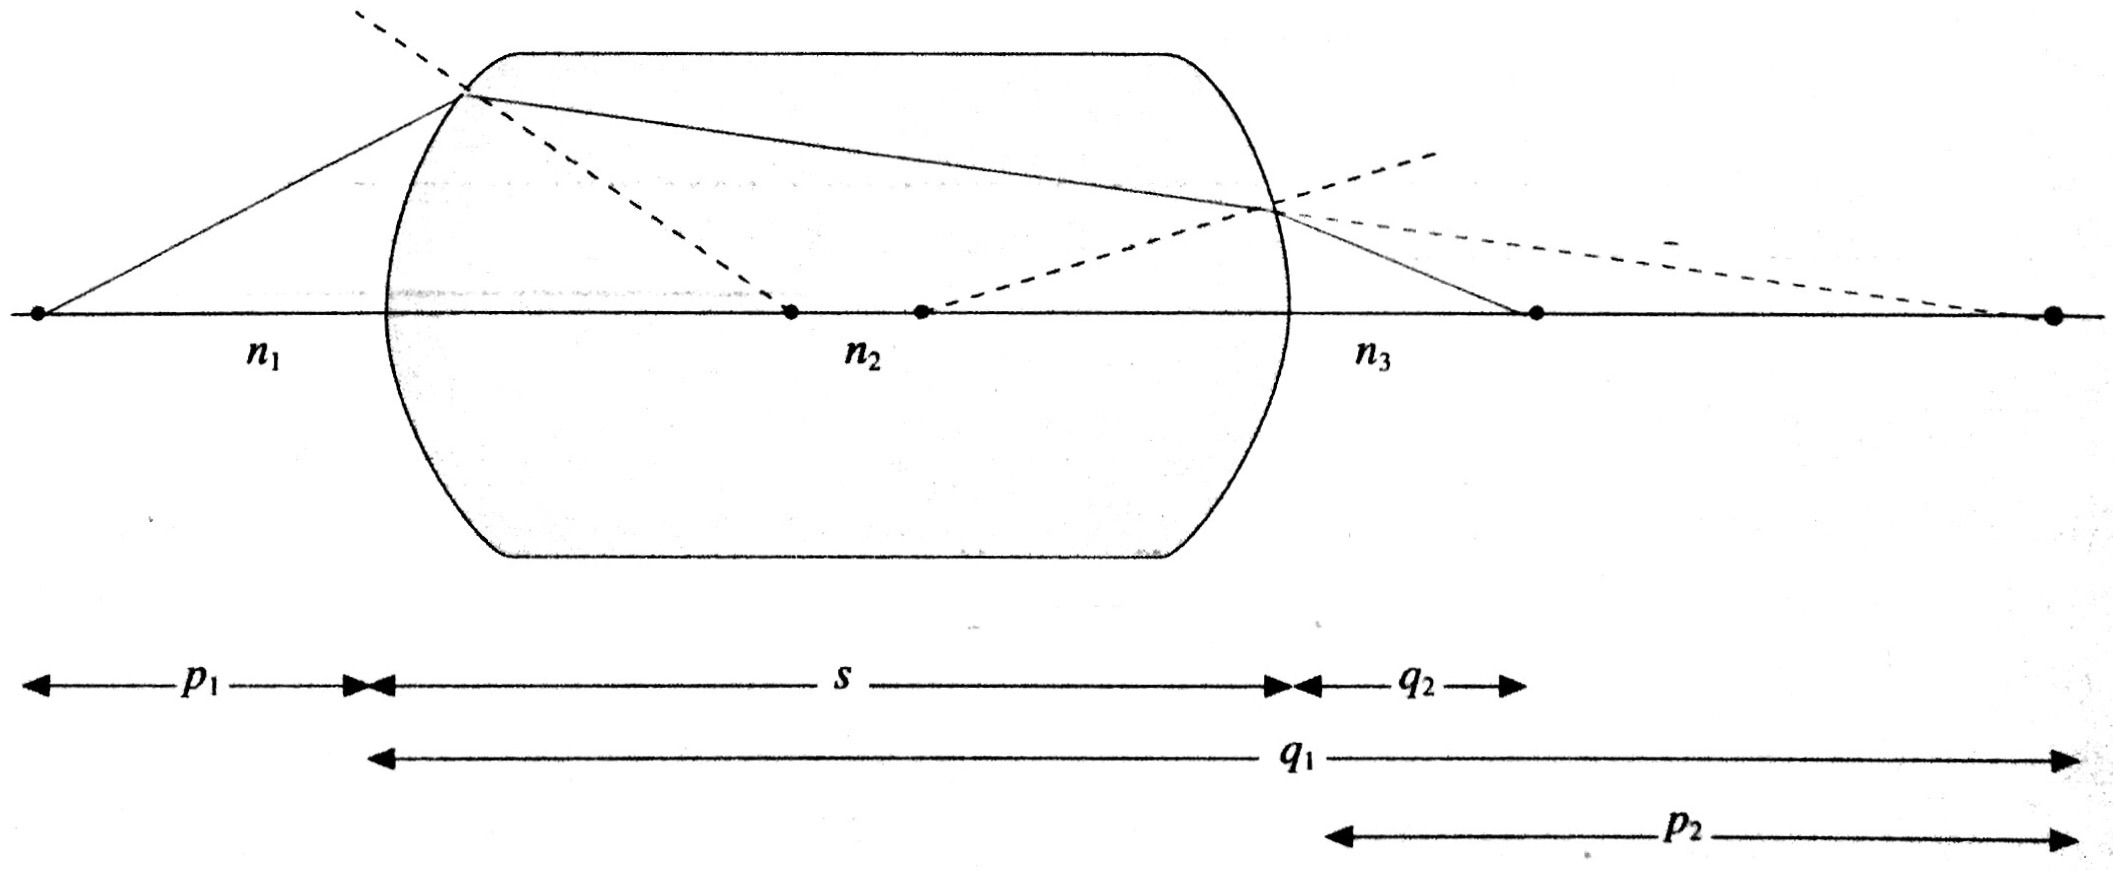
\includegraphics[width=\textwidth]{immagini/lentisottili1.jpg}
\end{center}

Due superfici diottriche aventi lo stesso asse individuano tre regioni distinte: la luce proveniente da sinistra si propaga nel primo mezzo avente indice di rifrazione $\n1$, viene trasmessa dal primo diottro e attraverso il mezzo con indice di rifrazione $\n2$ e infine, dopo la trasmissione al secondo diottro, si propaga nel mezzo con indice di rifrazione $\n3$.

Il blocco di materiale trasparente con indice di rifrazione $\n2$ delimitato dalle due superfici diottriche viene chiamata \b{lente semplice}. La \b{lente sottile} implica che le superfici diottriche siano molto vicine.

Le \b{equazioni che descrivono il sistema} sono:
\begin{equation}\begin{split}
\frac{\n1}{p_1}+\frac{\n2}{q_1}=\frac{\n2-\n1}{R_1}, \qquad \frac{\n2}{p_2}+\frac{\n3}{q_2}=\frac{\n3-\n2}{R_2}
\end{split}\end{equation}

Ponendo $s=0$ e $\n3=\n1$ si ottiene:
\begin{equation}\begin{split}
\frac{\n1}{p_1}+\frac{\n1}{q_2}=\(\n2-\n1\)\(\frac{1}{R_1}-\frac{1}{R_2}\)
\end{split}\end{equation}
perché i vertici dei diottri sono praticamente coincidenti tra loro e col centro della lente, $p_1$ e $q_2$ sono le distanze dell'oggetto e dell'immagine finale dal centro della lente. Si pone inoltre la \b{distanza focale}:
\begin{equation}\begin{split}
\frac{1}{f}=\frac{\n2-\n1}{\n1}\(\frac{1}{R_1}-\frac{1}{R_2}\)\\
\Longrightarrow f=\frac{\n1}{\n2-\n1}\frac{R_1R_2}{R_2-R_1}
\end{split}\end{equation}
che porta all'\b{equazione della lente sottile}:
\begin{equation}\begin{split}
\frac{1}{p}+\frac{1}{q}=\frac{1}{f}.
\end{split}\end{equation}
definendo $\frac{1}{f}$ il \b{potere convergente} (positivo se convergente, negativo se divergente).

Se l'\b{oggetto è posto all'infinito}, l'immagine si forma nel punto $F_2$ a distanza $f$ dal centro, mentre se l'\b{oggetto è posto nel punto $F_1$ a distanza $f$ dal centro}, l'immagine si forma all'infinito.

Sono convergenti le lenti più spesse al centro che al bordo, divergenti quelle più sottili al centro che al bordo. Se $\n2<\n1$ i ruoli si scambiano: essendo in generale una lente fatta di vetro e immersa in aria, il caso $\n2>\n1$ è quello più comune. Quando $R_2=-R_1$, la lente è detta \b{simmetrica} e la sua focale vale:
\begin{equation}\begin{split}
f=\frac{\n1}{\n2-\n1}\frac{R}{2}.
\end{split}\end{equation}

\subsubsection{Relazioni tra oggetto e immagine}
\begin{center}
\begin{tabularx}{\textwidth}{Xc| Xc |c}
\toprule
\multicolumn{2}{c}{Oggetto} 			& \multicolumn{2}{c}{Immagine} 				& \\
\midrule
$+\infty\ge p\ge f$ 		& reale 		& $f\le q\le +\infty$ 			& reale 		& \\[2ex]
$f\ge p\ge 0$ 			& reale 		& $-\infty\le q\le 0$ 			& virtuale 		& $\frac{1}{f}>0$ \\[2ex]
$0\ge p\ge -\infty$ 		& virtuale 		& $0\le q \le f$ 				& reale 		& \\[2ex]
\midrule
$+\infty\ge p\ge 0$ 		& reale 		& $f\le q\le 0$ 				& virtuale 		& \\[2ex]
$0\ge p\ge f$ 			& virtuale 		& $0\le q\le +\infty$ 			& reale 		& $\frac{1}{f}<0$ \\[2ex]
$f\ge p\ge -\infty$ 		& virtuale 		& $-\infty\le q \le f$ 			& virtuale 		& \\[2ex]
\bottomrule
\end{tabularx}
\end{center}

Si ricava l'espressione dell'\b{ingrandimento trasversale}:
\begin{equation}\begin{split}
\In=\frac{y}{x}=\frac{q-f}{f}=\frac{f}{p-f}=\frac{q}{p}
\end{split}\end{equation}
e dell'\b{ingrandimento longitudinale}:
\begin{equation}\begin{split}
\frac{\Delta q}{\Delta p}=-I_1I_2.
\end{split}\end{equation}

